% $Id: Note_ResFit_ToyMC.tex,v 1.4 2010/07/08 14:32:36 mschrode Exp $


\section{Study with a Toy Monte Carlo Simulation}\label{sec:ResFit:ToyMC}

The method presented in the previous Section~\ref{sec:ResFit:Method}
is studied using a simple simulation, \textit{Toy Monte Carlo}.
First, the basic likelihood fit described in
Section~\ref{sec:ResFit:Method:Likelihood} is performed (Section~\ref{sec:ResFit:ToyMC:PtGenCuts}),
whereby events have been selected using Monte Carlo truth information.
Second, a data driven event selection has been applied and the
modified likelihood, described in
Section~\ref{sec:ResFit:Method:Biases}, is maximised (Section~\ref{sec:ResFit:ToyMC:PtCaloCuts}).


\subsection{Generated sample}\label{sec:ResFit:ToyMC:Sample}

A sample of $30\,000$ ideal dijet events has been generated assuming a
simple exponential particle level jet \pt spectrum
\begin{equation}
  \label{eq:ResFit:ToyMC:Spectrum}
  f\left(\pttrue\right) \propto \exp\left(-\pttrue / \tau\right),
  \qquad \tau = 80.
\end{equation}
ranging from \mbox{$50 < \pttrue < 1000\gev$} (comp. Fig.~\ref{fig:ResFit:ToyMC:Sample:Spectrum}).
Two independent measurements of the jet \pt have been simulated by
weighting \pttrue with random numbers drawn from a Gaussian response
\begin{equation}
  \label{eq:ResFit:ToyMC:Response}
  r_{\mathbf{\xi}}\left(\ptmeas|\pttrue\right) = 
  \frac{1}{\sqrt{2\pi}\sigma}\exp\left[-\frac{1}{2}\left(\frac{\ptmeas - \pttrue}{\sigma}\right)^{2}\right]
\end{equation}
(Here and in the following the jet index $i$ has been omitted.)
The standard deviation, i.e. the jet resolution, $\sigma$ has been parametrised as a function of \pttrue and
the parameters $\xi_{i}$, \mbox{$i\in [0,2]$}, as
\begin{equation}
  \label{eq:ResFit:ToyMC:Sigma}
  \sigma = \xi_{0}\gev
  \oplus \xi_{1}\,\sqrt{\pt\gev}\oplus \xi_{2}\pt.
\end{equation}
The values of the parameters $\mathbf{\xi}$ are listed in
Tab.~\ref{tab:ResFit:ToyMC:PtGenCuts:FitResult}.
An example of a simulated response distribution is shown in Fig. ~\ref{fig:ResFit:ToyMC:PtGenCuts:Response}.

\begin{figure}[ht]
  \centering
  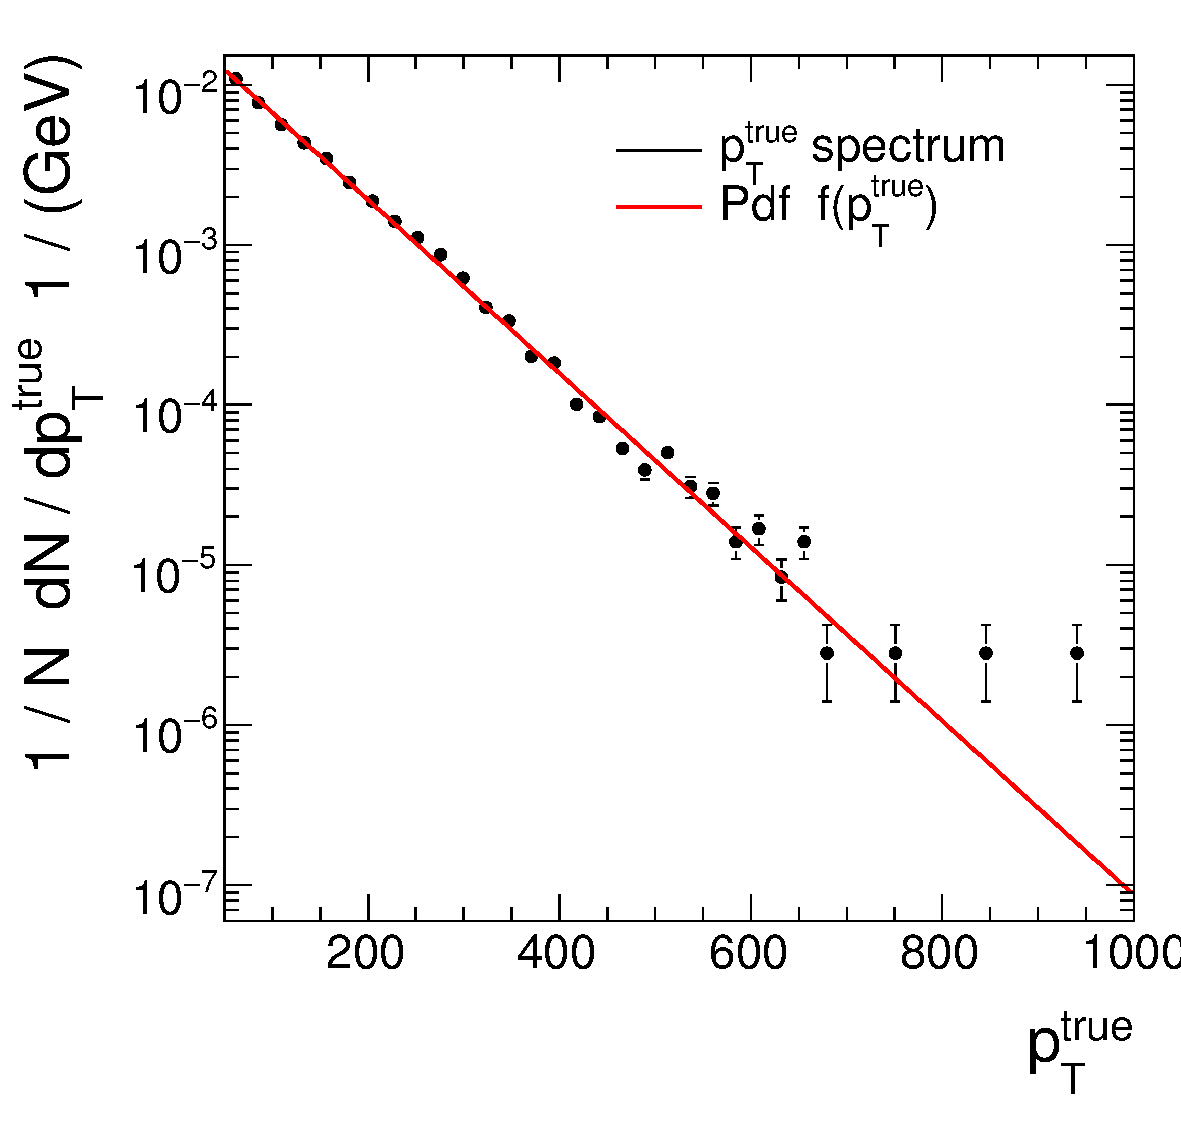
\includegraphics[width=0.45\textwidth]{figures/resFit_ToyMC_PtGenCuts_SpectrumLog}
  \caption{Toy Monte Carlo simulation of a sample of ideal dijet events.
    Generated \pttrue spectrum (circular markers) and the underlying pdf (solid line).}
  \label{fig:ResFit:ToyMC:Sample:Spectrum}
\end{figure}


\subsection{Measurement of the resolution with a truth information based event selection}\label{sec:ResFit:ToyMC:PtGenCuts}

The jet energy resolution of the dijet sample is to be measured as described in Section~\ref{sec:ResFit:Method:Likelihood}.
Dijet events are have been selected from the sample described above by
requiring \mbox{$\ptmin < \pttrue < \ptmax$}.
The jet \pt spectrum is taken directly from the
simulation~\eqref{eq:ResFit:ToyMC:Spectrum}, while the jet \pt
response is assumed to be Gaussian and the resolution $\sigma$ to
depend on \pttrue and the parameters $\mathbf{\xi}$ as
in~\eqref{eq:ResFit:ToyMC:Sigma}.

\begin{figure}[ht]
\centering
\begin{tabular}{cc}
  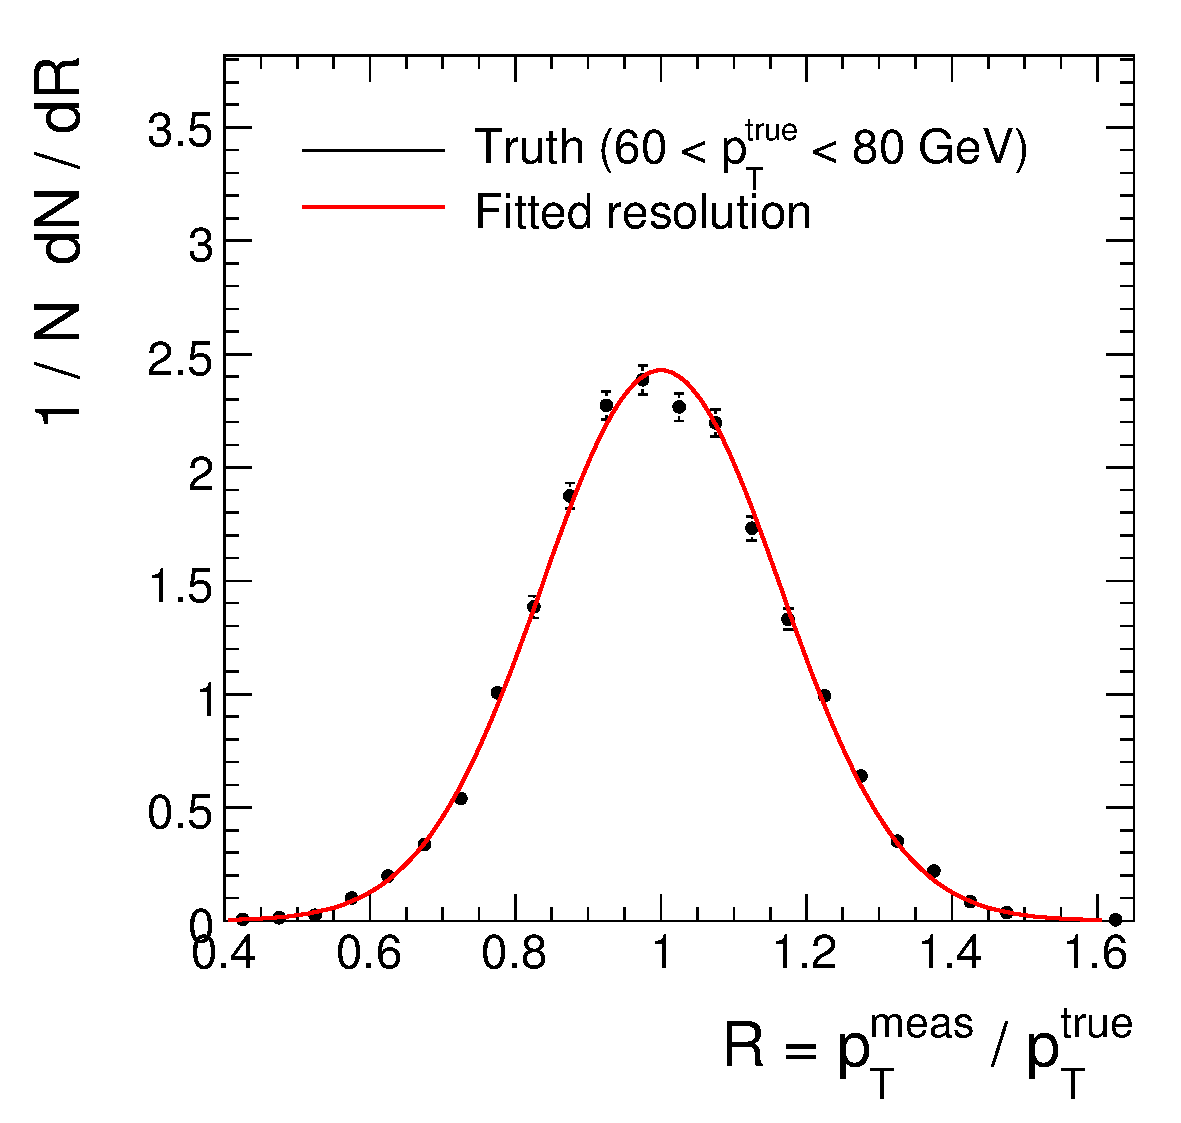
\includegraphics[width=0.45\textwidth]{figures/resFit_ToyMC_PtGenCuts_ResolutionBin1} &
  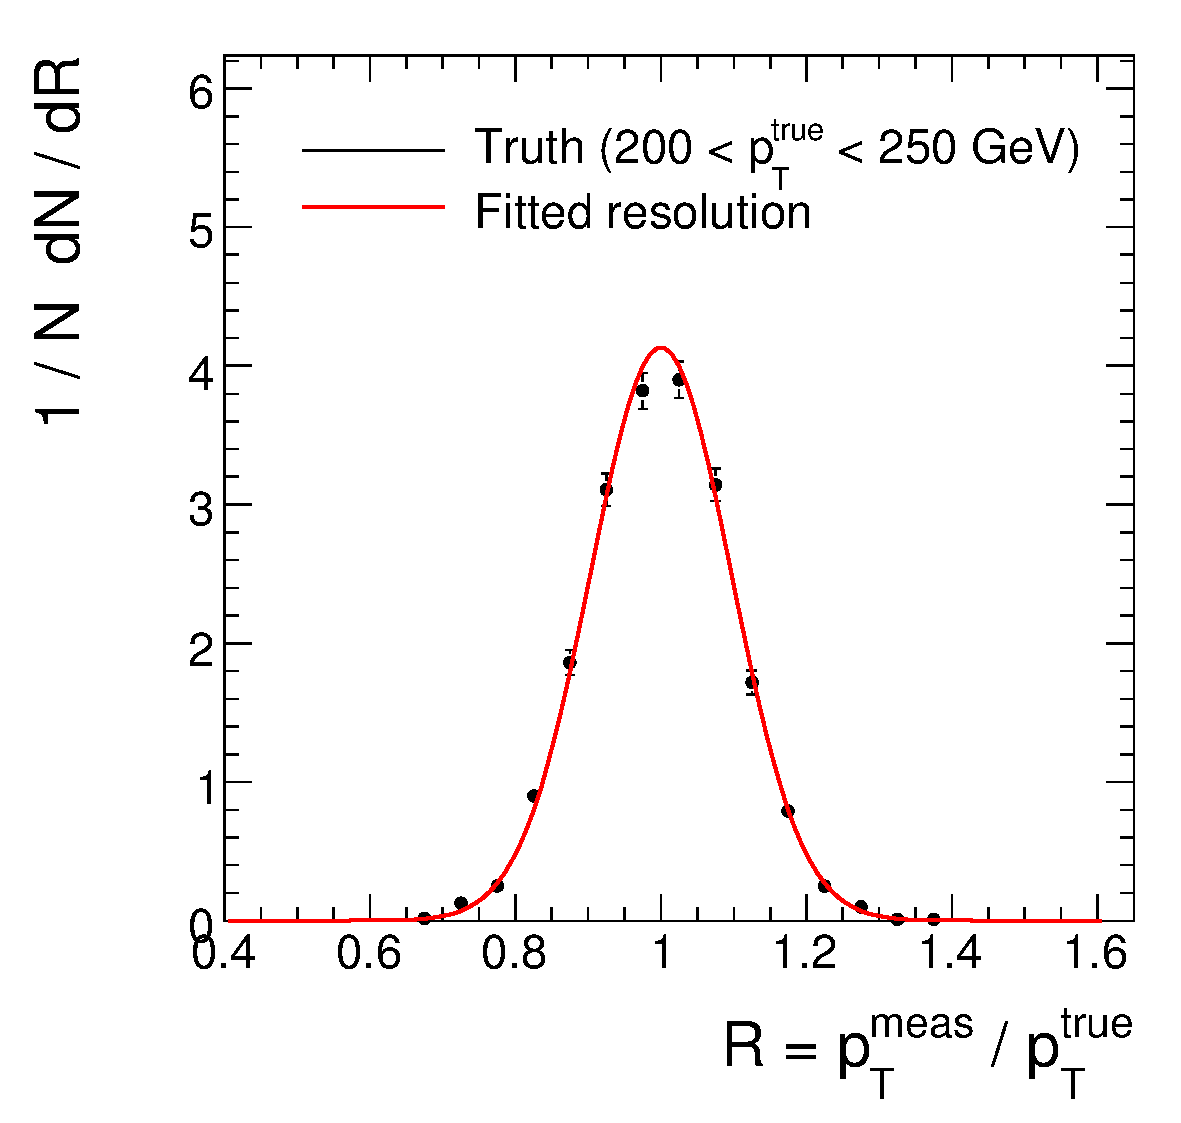
\includegraphics[width=0.45\textwidth]{figures/resFit_ToyMC_PtGenCuts_ResolutionBin7} \\      
\end{tabular}
\caption{Simple simulation of a sample of ideal dijet events.
  Generated true response \mbox{$\ptmeas / \pttrue$} (histogram) and
  the response (solid line) from the maximum likelihood fit in two
  different \pttrue bins.
  The latter has been evaluated for the mean \pttrue in these bins.
  Note, here ``fit'' does not refer to a fit to the shown histogram but the maximisation of the likelihood~\eqref{eq:ResFit:Likelihood}.
}
\label{fig:ResFit:ToyMC:PtGenCuts:Response}
\end{figure}


\begin{table}[ht]
  \caption{Parameter values of the Gaussian jet \pt resolution
    $\sigma$.
    Listed are the true values used for the generation and
    the fitted values.
    The uncertainties assigned to the fitted values
    are the statistical uncertainties from the fit.
    The parameter correlations are shown in Fig.~\ref{fig:ResFit:ToyMC:PtGenCuts:ParCorr}.}
  \centering
  \begin{tabular}[ht]{lccc}
    \toprule
    $\xi_{i}$ & $0$ & $1$ & $2$ \\
    \midrule
    True value & $4$           & $1.2$           & $0.05$ \\
    Fit result & $4.5 \pm 0.7$ & $1.18 \pm 0.05$ & $0.051 \pm 0.004$ \\
    \bottomrule
  \end{tabular}
  \label{tab:ResFit:ToyMC:PtGenCuts:FitResult}
\end{table}


\begin{figure}[ht]
  \centering
  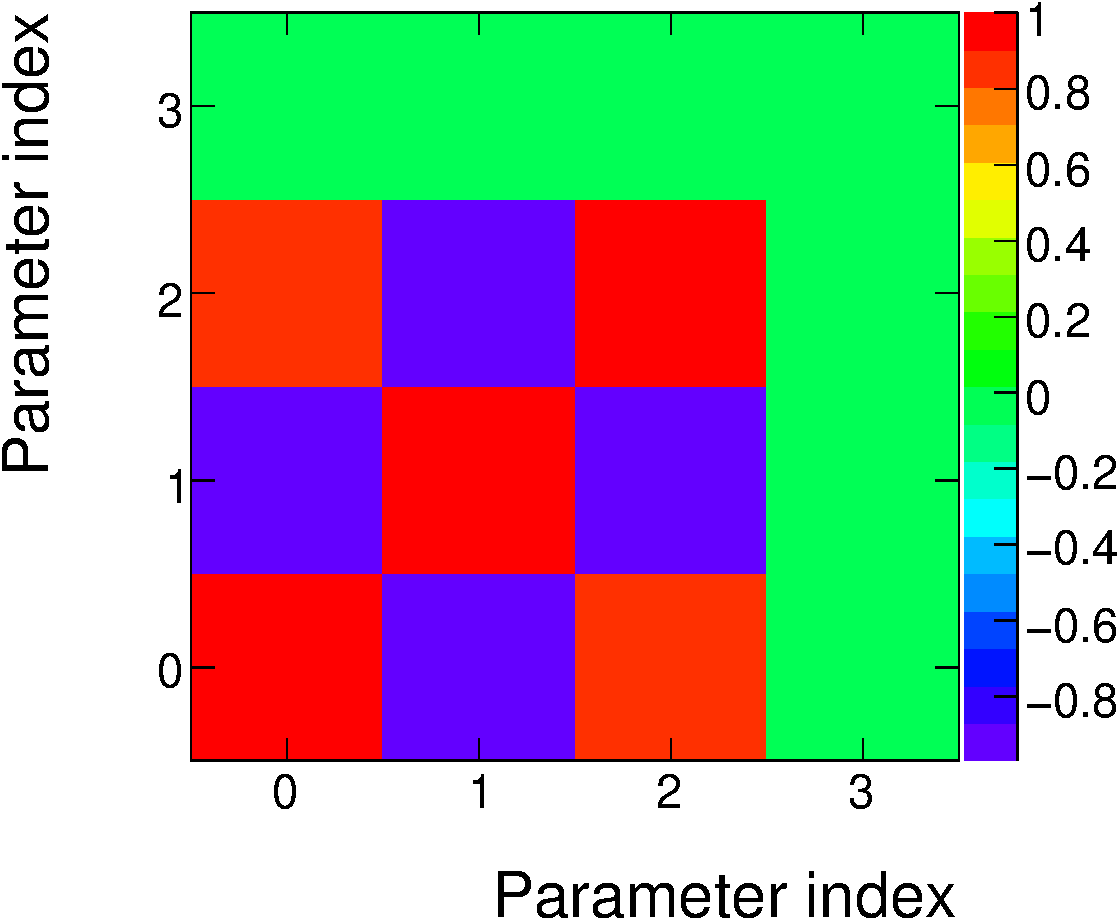
\includegraphics[width=0.45\textwidth]{figures/resFit_ToyMC_PtGenCuts_Correlations}
  \caption{Correlation coefficients of the fitted parameter values
    $\mathbf{\xi}$ of the Gaussian jet \pt resolution $\sigma$. 
    Parameter $3$ corresponds to the slope $\tau$ of the
    spectrum, which is fixed during the fit, and is to be ignored.}
  \label{fig:ResFit:ToyMC:PtGenCuts:ParCorr}
\end{figure}

The fitted parameter values $\mathbf{\xi}$ are listed in Tab.~\ref{tab:ResFit:ToyMC:PtGenCuts:FitResult};
they agree with the true values within the statistical uncertainties.

The parameters are strongly (anti-) correlated (comp. Fig.~\ref{fig:ResFit:ToyMC:PtGenCuts:ParCorr}).
In the present \pttrue interval from \mbox{$\ptmin = 50\gev$} to \mbox{$\ptmax = 1000\gev$}, the used parametrisation of the Gaussian resolution $\sigma$ is over-determined.
The $\xi_{0}$ term in~\eqref{eq:ResFit:ToyMC:Sigma} is most important at very low \pt while the $\xi_{2}$ term dominates at very large \pt.
Hence, omitting either the terms with $\xi_{0}$ and $\xi_{2}$ or the
term with $\xi_{1}$ would have been sufficient to describe the measured events.

\begin{figure}[ht]
  \centering
  \begin{tabular}{cc}
    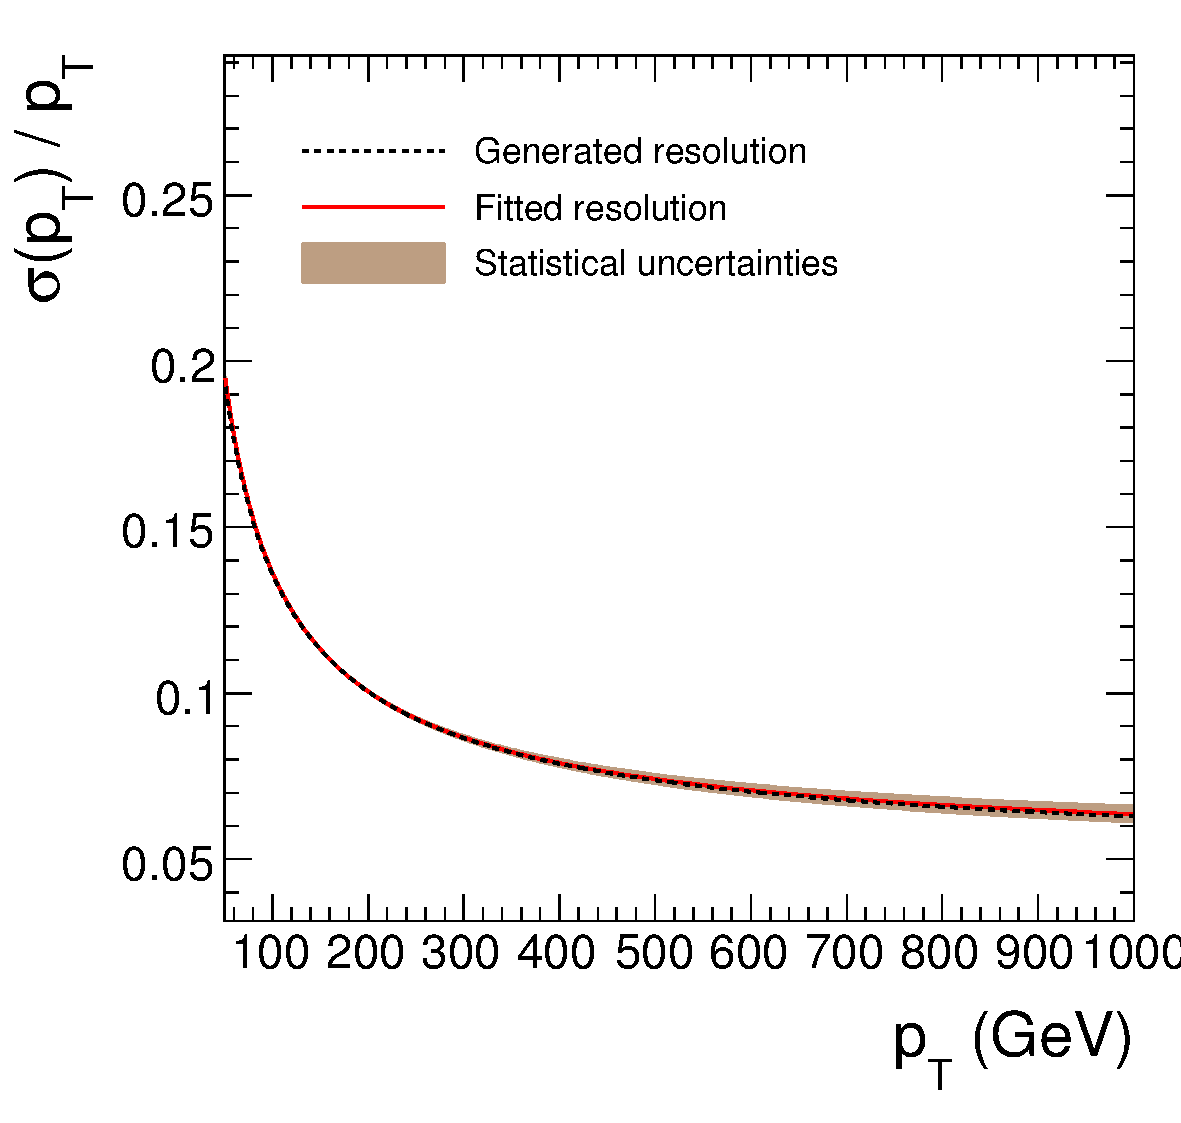
\includegraphics[width=0.45\textwidth]{figures/resFit_ToyMC_PtGenCuts_Sigma} &
    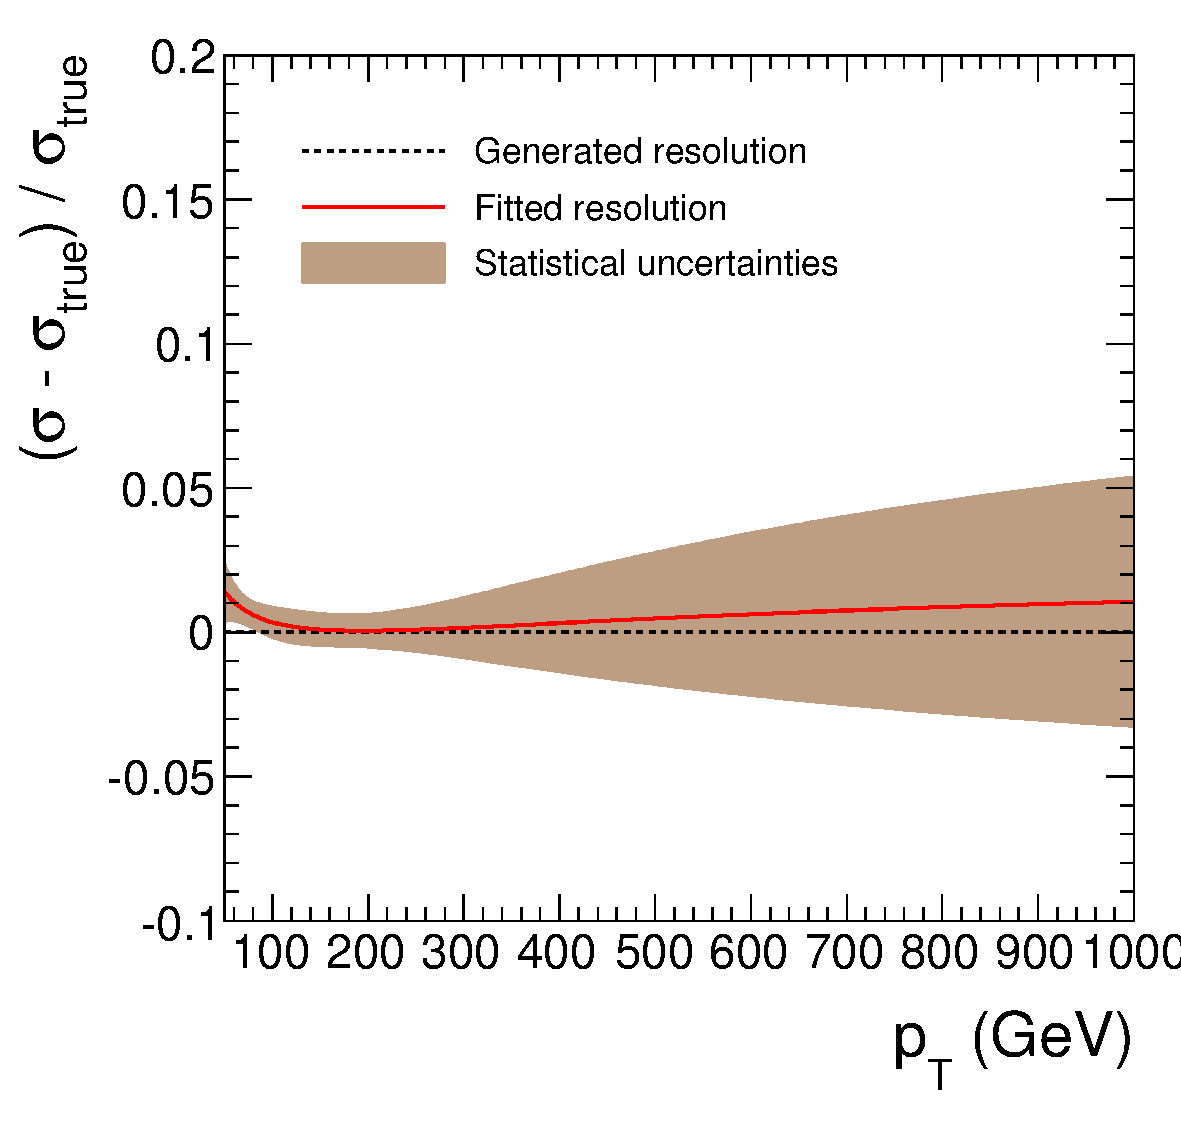
\includegraphics[width=0.45\textwidth]{figures/resFit_ToyMC_PtGenCuts_SigmaRelDifference} \\
  \end{tabular}
  \caption{(\textit{Left}) Relative Gaussian resolution $\sigma(\pt)/\pt$ evaluated with the fitted
    parameter values (solid line) in comparison to the true resolution
    (dashed line) and (\textit{right}) the relative difference
    $\sigma_{\text{fit}} / \sigma_{\text{true}}$.
    The shaded areas represent the propagated statistical
    uncertainty on the fitted parameter values, taking into account the
    parameter correlations.}
  \label{fig:ResFit:ToyMC:PtGenCuts:FittedSigma}
\end{figure}

The Gaussian resolution $\sigma(\pt)/\pt$ evaluated with the fitted
parameter values is shown in Fig.~\ref{fig:ResFit:ToyMC:PtGenCuts:FittedSigma}
in comparison to the true width at generation.
There is good agreement between the fitted and the true resolution.
The uncertainties are about $1\%$ at low \pt rising to
about $3\%$ at $\pt \approx 600\gev$ where there is sufficient statistics in
the generated sample (comp. Fig~\ref{fig:ResFit:ToyMC:Sample:Spectrum}).
For larger \pt the uncertainties rise up to $4.5\%$.

An example of the resulting response distribution in comparison to the true
distribution is shown in Fig.~\ref{fig:ResFit:ToyMC:PtGenCuts:Response} for
two different \pttrue bins.


\subsection{Measurement of the resolution with a data driven event
  selection}\label{sec:ResFit:ToyMC:PtCaloCuts}

The modification of the maximum likelihood method for a data driven
event selection discussed in Section~\ref{sec:ResFit:Method:Biases} is
tested using the Toy Monte Carlo simulation.
Events are selected by requiring the measured \pt of the
first\footnote{This is that one jet of the two leading jets the
  selection requirement is placed on, i.e. not necessarily the leading
  jet (comp. Section~\ref{sec:ResFit:Method:Biases}).} jet to
meet \mbox{$\ptmin = 80 < \ptmeasi{1} < \ptmax = 800\gev$} (comp. Fig.~\ref{fig:ResFit:ToyMC:PtCuts:Spectrum}).

\begin{figure}[ht]
  \centering
  \begin{tabular}{cc}
    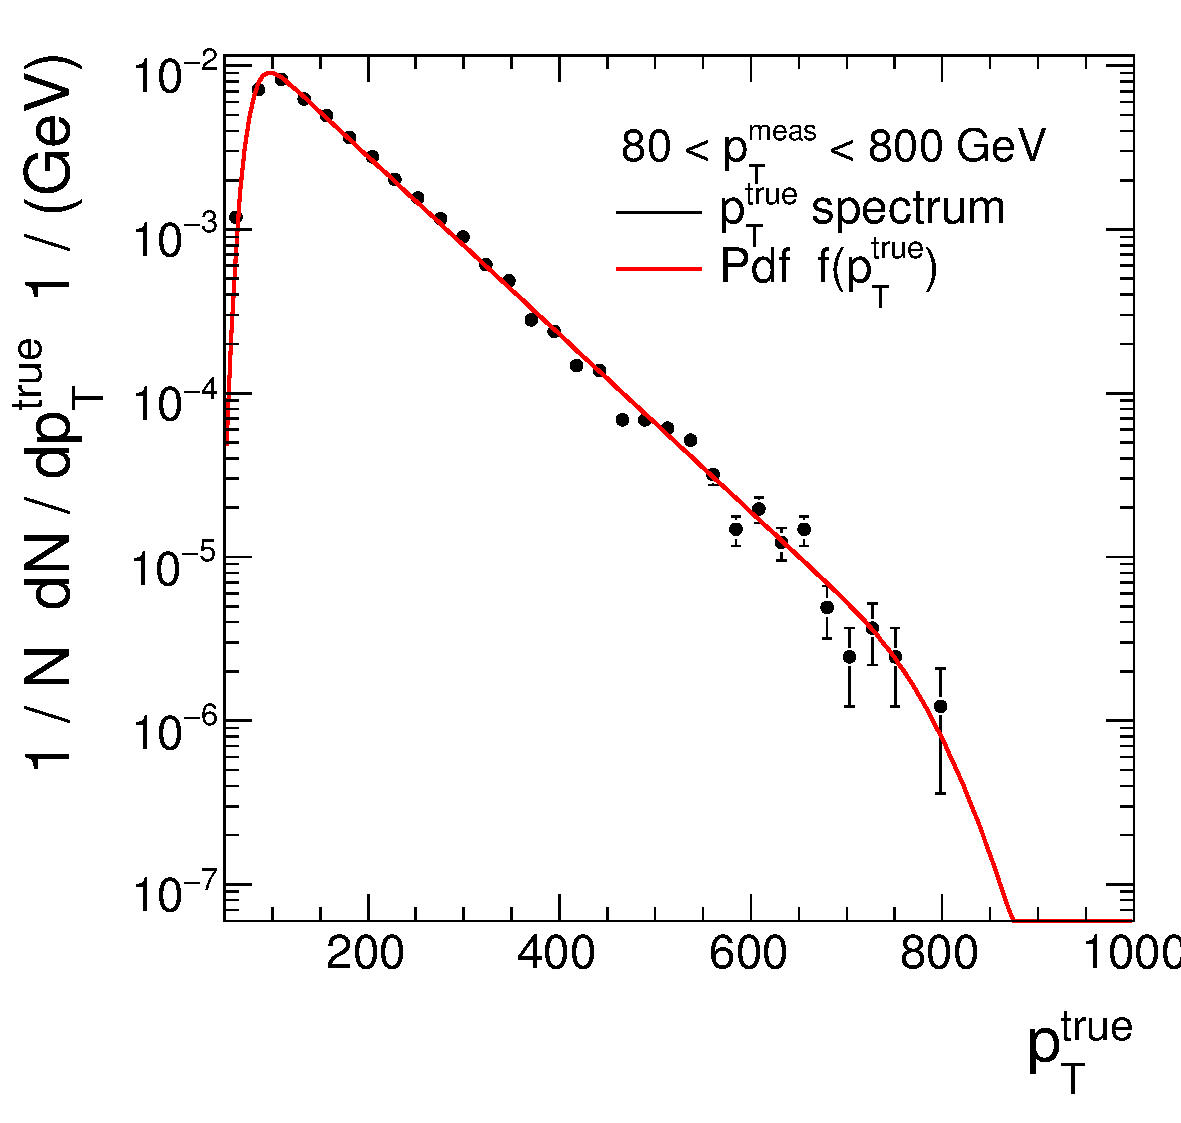
\includegraphics[width=0.45\textwidth]{figures/resFit_ToyMC_PtCuts_SpectrumLog} &
    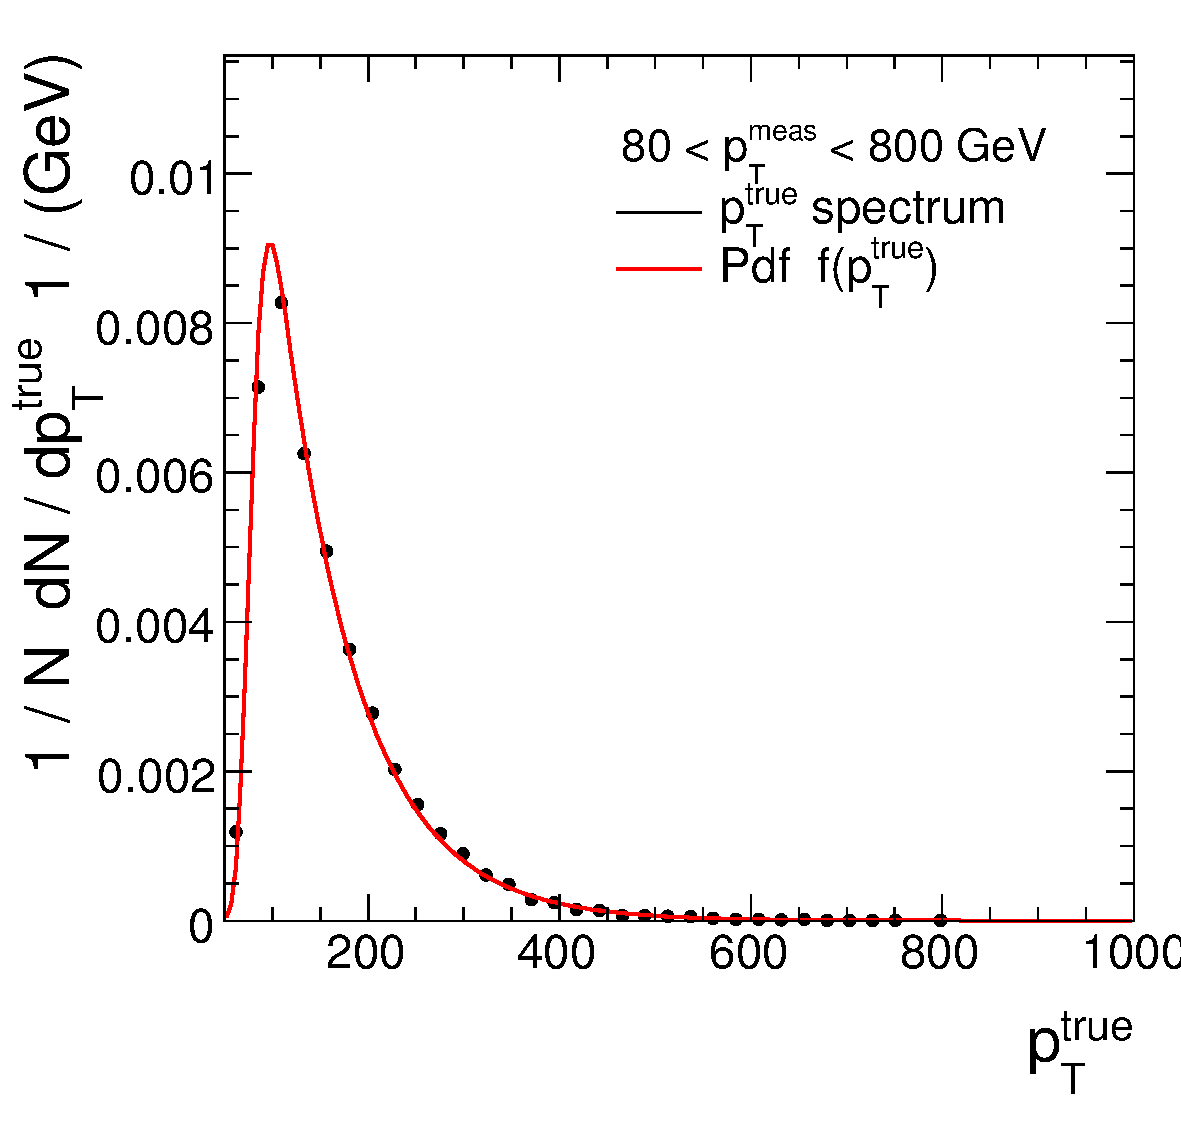
\includegraphics[width=0.45\textwidth]{figures/resFit_ToyMC_PtCuts_SpectrumLinear} \\
  \end{tabular}
  \caption{Demonstration of the migration effects caused by a data
    driven event selection.
    Shown is the \pttrue spectrum (circular markers) after
    requiring \mbox{$80 < \ptmeas < 800\gev$}, in linear scale
    (\textit{left}) and logarithmic scale scale (\textit{right}).
    The spectrum is well described by the modified pdf
    $\tilde{f}(\pttrue)$.
    (Compare the underlying spectrum Fig.~\ref{fig:ResFit:ToyMC:Sample:Spectrum}.)
  }
  \label{fig:ResFit:ToyMC:PtCuts:Spectrum}
\end{figure}


\begin{figure}[ht]
  \centering
  \begin{tabular}{cc}
    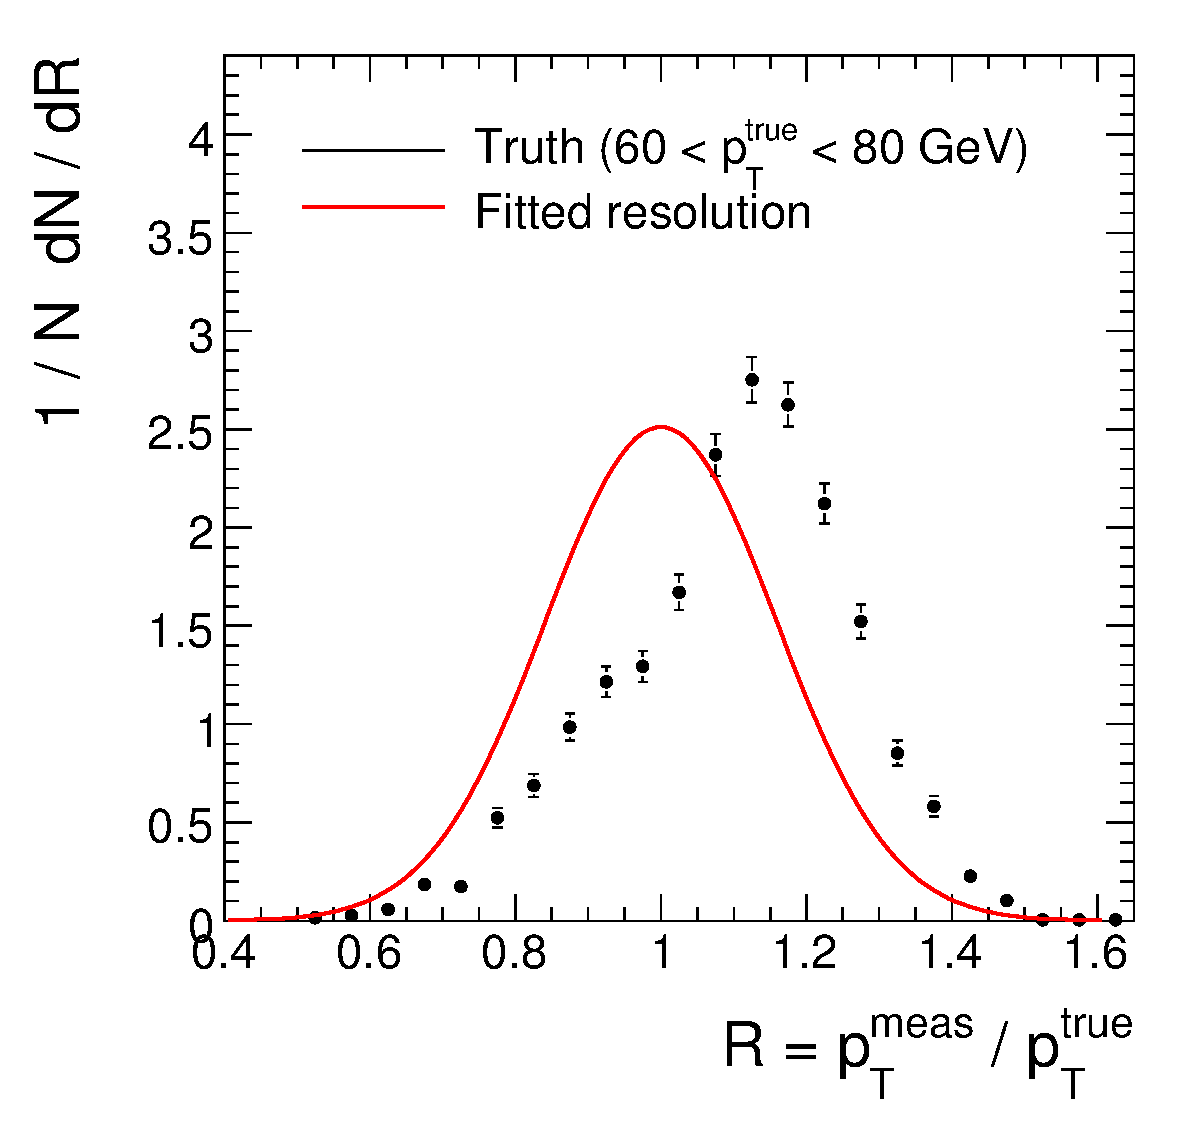
\includegraphics[width=0.45\textwidth]{figures/resFit_ToyMC_PtCuts_ResolutionBin1} &
    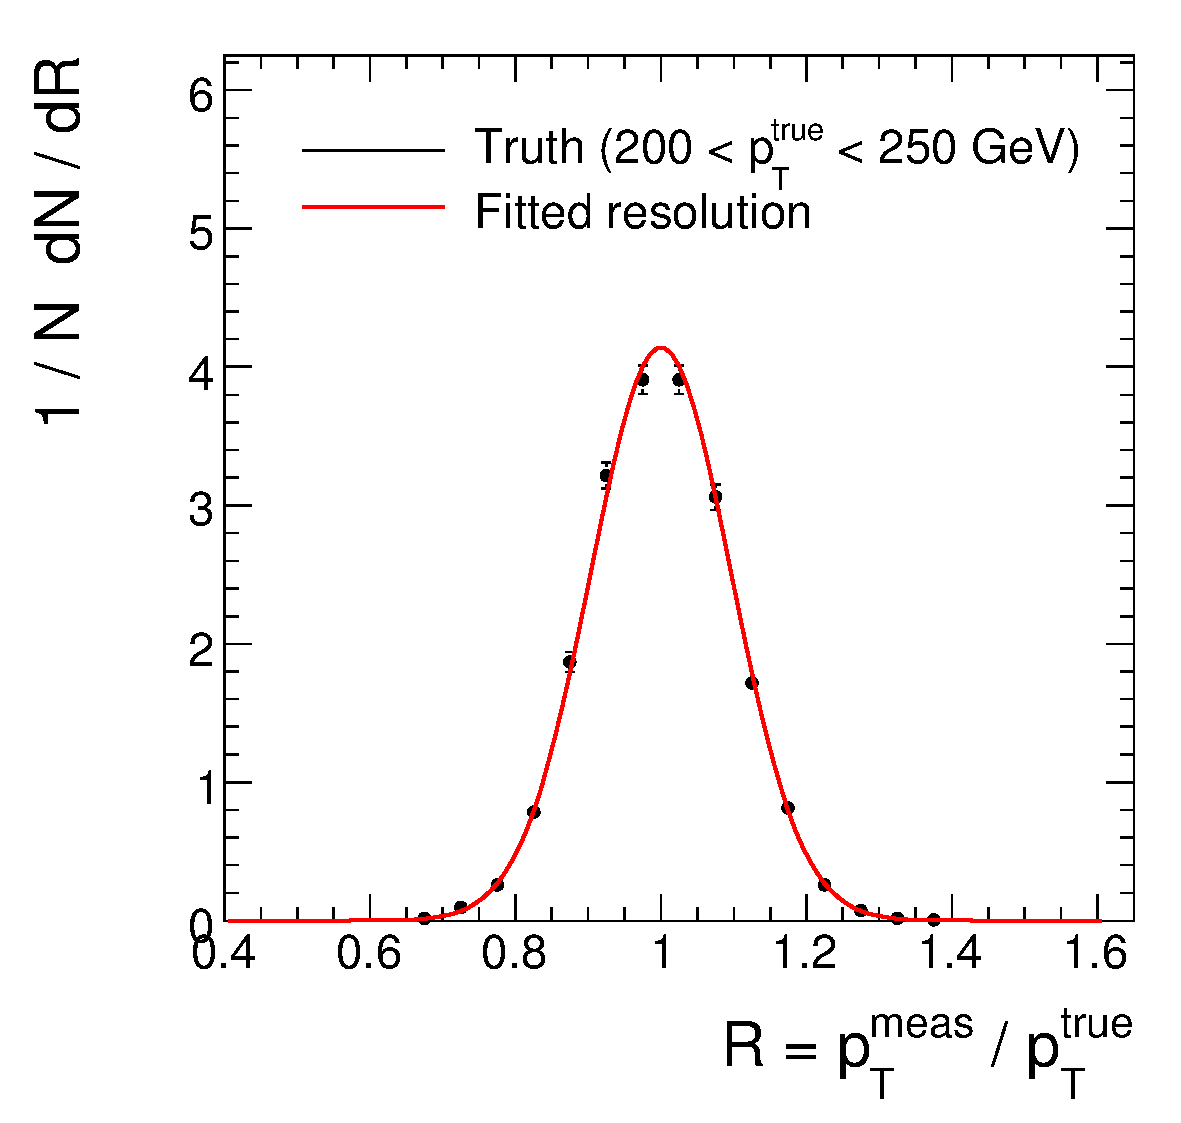
\includegraphics[width=0.45\textwidth]{figures/resFit_ToyMC_PtCuts_ResolutionBin7} \\
  \end{tabular}
  \caption{Generated Gaussian response \mbox{$\ptmeas / \pttrue$}
    (circular markers) and the fitted
    response (solid line) in two different \pttrue bins after
    requiring \mbox{$80 < \ptmeas < 800\gev$}.
    Note the migration effects (\textit{left}): the narrow peak at the
    right side is populated by the first jets in each event, i.e. that have been cut on, and hence these are jets fluctuating upwards into the \pt bin.
    The wider peak centred around 1 is populated by the unconstrained
    second jet.
    (There is more upward than downward fluctuation due to the falling
    \pttrue spectrum.)
  }
  \label{fig:ResFit:ToyMC:PtCuts:Response}
\end{figure}

\begin{figure}[ht]
  \centering
  \begin{tabular}{cc}
    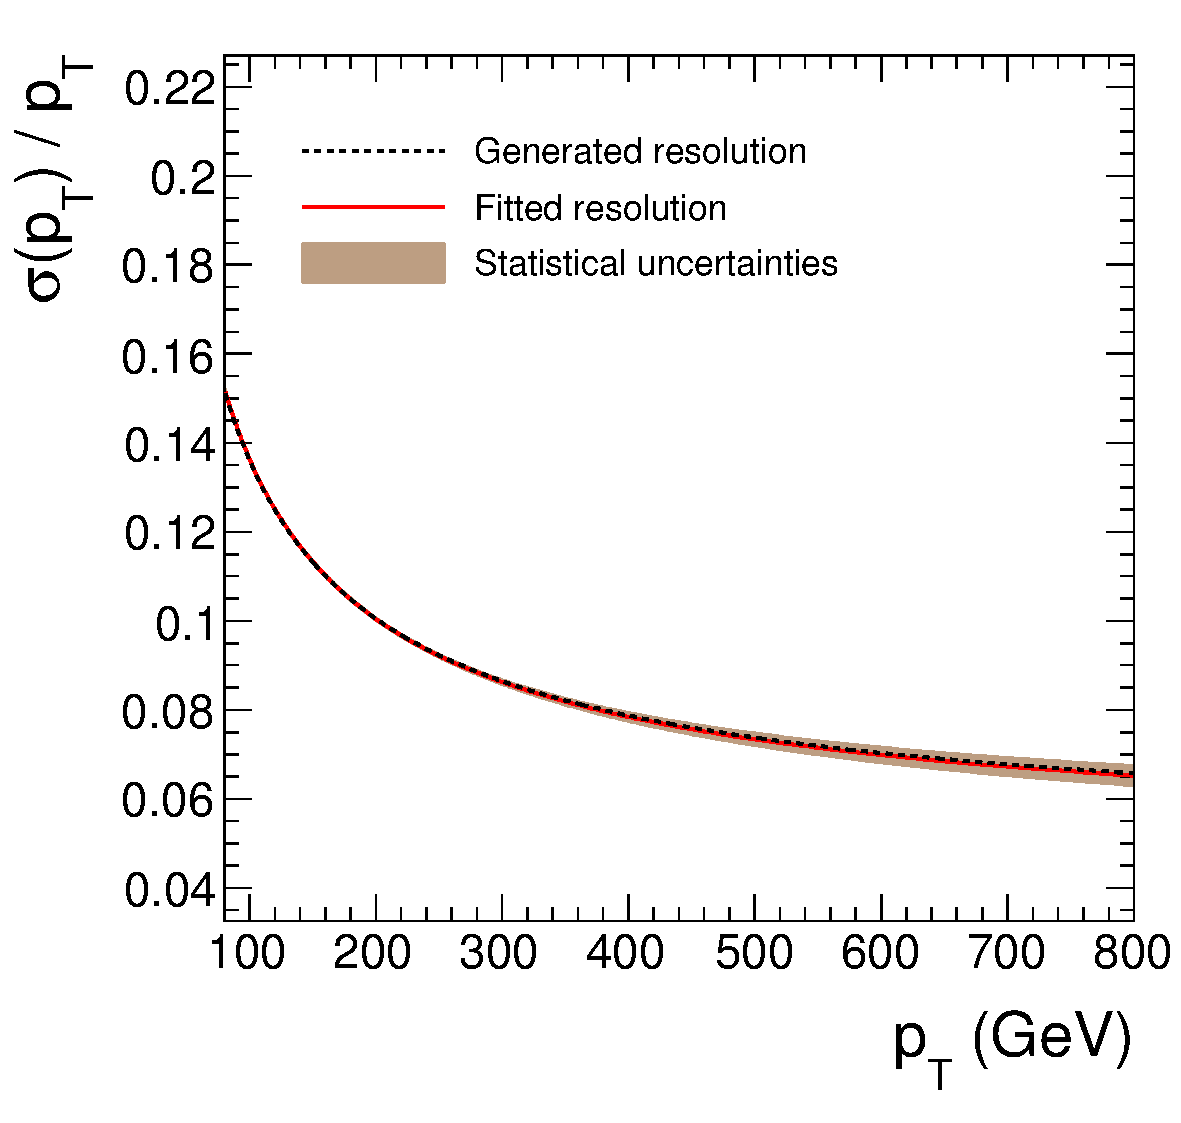
\includegraphics[width=0.45\textwidth]{figures/resFit_ToyMC_PtCuts_Sigma} &
    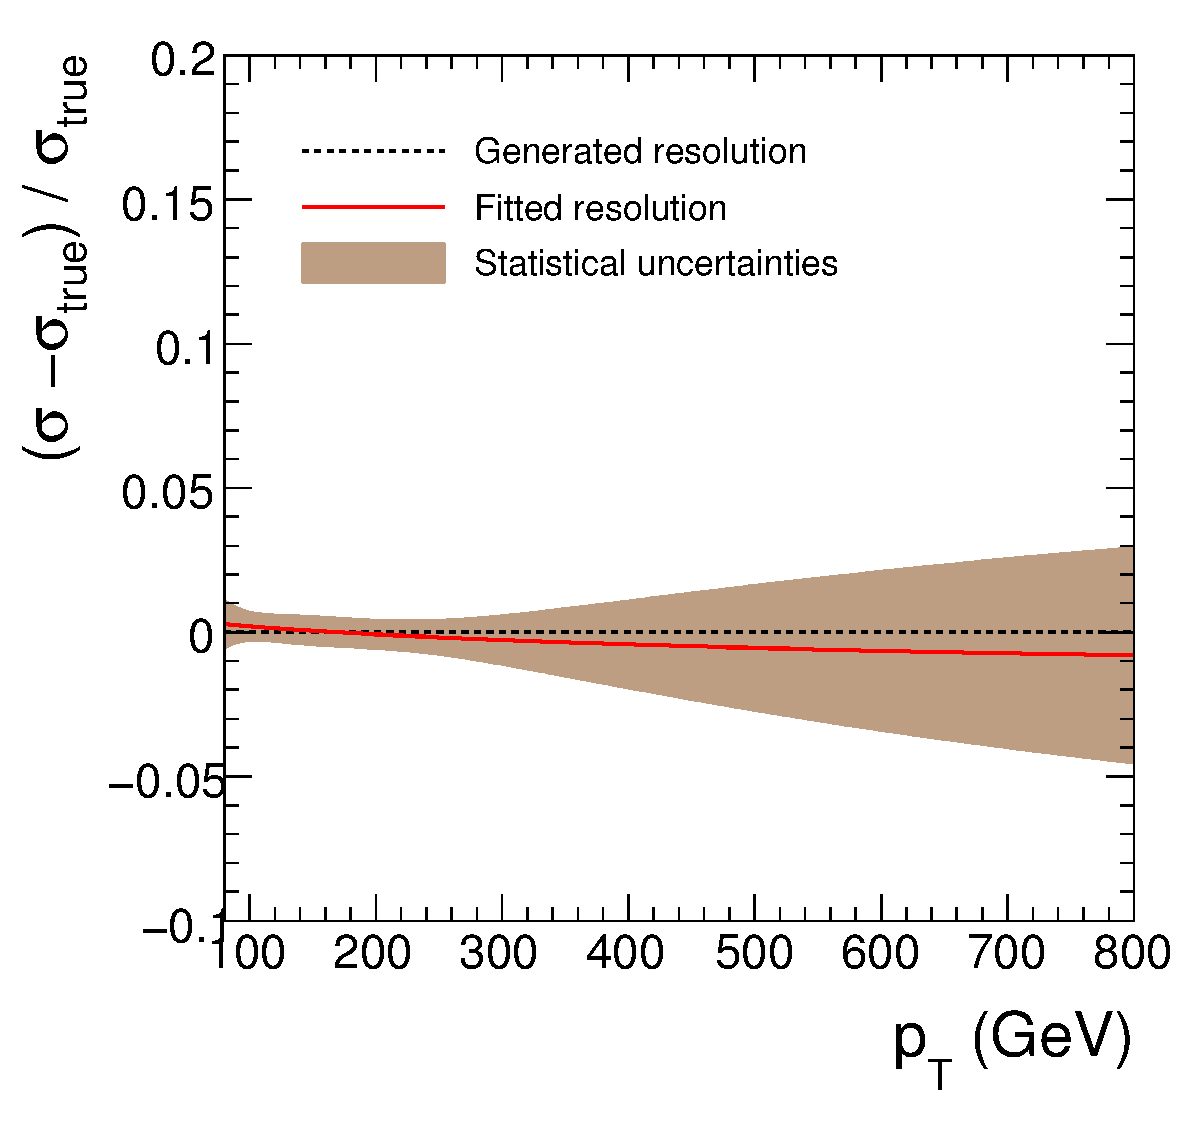
\includegraphics[width=0.45\textwidth]{figures/resFit_ToyMC_PtCuts_SigmaRelDifference} \\
  \end{tabular}
  \caption{(\textit{Left}) Relative Gaussian resolution $\sigma(\pt)/\pt$ evaluated with the fitted
    parameter values (solid line) in comparison to the true resolution
    (dashed line) and (\textit{right}) the relative difference
    $\sigma_{\text{fit}} / \sigma_{\text{true}}$.
    The shaded areas represent the propagated statistical
    uncertainty on the fitted parameter values, taking into account the
    parameter correlations.
    The fit has been performed with dijet events selected by requiring \mbox{$80 < \ptmeas < 800\gev$}.}
  \label{fig:ResFit:ToyMC:PtCuts:FittedSigma}
\end{figure}


\begin{table}[ht]
  \caption{Parameter values of the Gaussian jet \pt resolution
    $\sigma$.
    Listed are the true values used for the generation and
    the fitted values.
    The uncertainties assigned to the fitted values
    are the statistical uncertainties from the fit.
    The fit has been performed with dijet events selected by requiring \mbox{$80 < \ptmeas < 800\gev$}.}
  \centering
  \begin{tabular}[ht]{lccc}
    \toprule
    $b_{i}$ & $0$ & $1$ & $2$ \\
    \midrule
    True value & $4$           & $1.2$                   & $0.05$ \\
    Fit result   & $4 \pm 1$ & $1.20 \pm 0.07$ & $0.049 \pm 0.005$ \\
    \bottomrule
   \end{tabular}
 \label{tab:ResFit:ToyMC:PtCuts:FitResult}
\end{table}


The fitted parameter values $\mathbf{\xi}$ of the Gaussian resolution $\sigma$ are listed in Tab.~\ref{tab:ResFit:ToyMC:PtCuts:FitResult}.
They agree with the true values within the statistical uncertainties.
As expected, they feature the same correlation pattern as in the
fitted parameters in Section~\ref{sec:ResFit:ToyMC:PtGenCuts}.

The relative Gaussian resolution $\sigma(\pt)/\pt$ evaluated with the fitted parameter values is shown in Fig.~\ref{sec:ResFit:ToyMC:PtGenCuts} in comparison to the true resolution at generation.
There is good agreement within the statistical uncertainties.
As before, the uncertainties are about $1\%$ at low \pt rising to about $3\%$ at $\pt \approx 600\gev$ and up to $4.5\%$ at very large \pt.
An example of the resulting response distributions is shown in
Fig.~\ref{fig:ResFit:ToyMC:PtCuts:Response} for two \pttrue bins.

From the results presented in this section, it is concluded that the
maximum likelihood method is suited to measure the jet \pt resolution
of dijets that are perfectly balanced in \pttrue.